\cohead{\Large\textbf{Potenzfunktionen}}
\fakesubsection{Potenzfunktionen}
\setlength{\qrheight}{2.5cm}%
\newlength{\potenzfunktionenLength}%
\iftoggle{qrcode}{\setlength{\potenzfunktionenLength}{\textwidth-\qrheight}}{\setlength{\potenzfunktionenLength}{\textwidth}}%
\begin{minipage}{\textwidth}
\adjustbox{valign=t}{\begin{minipage}{\potenzfunktionenLength}
    Funktionen vom Typ
    \[f(x)=a\cdot x^n, \quad a\neq 0, \quad n\in\N\]
    bezeichnen wir als Potenzfunktionen.

    Der Koeffizient \(a\) ist der Streckfaktor, wie wir ihn bereits von quadratischen Funktionen kennen.

    Die Hochzahl bzw. der Exponent \(n\) ist eine natürliche Zahl: \(\N=\{1,\,2,\,3,\,4,\,\dots\}\)

    Die Schaubilder der Potenzfunktionen teilen sich in drei verschiedene Formen auf:
\end{minipage}}%
\iftoggle{qrcode}{%
    \adjustbox{valign=t}{\begin{minipage}{\qrheight}
            \href{https://www.geogebra.org/m/rp8rtgpv}{
\includegraphics[height=\qrheight]{\ganzFkt/pics/PotenzfunktionenQR.png}}%
    \end{minipage}}%
}{}%
\end{minipage}

\bigskip

\begin{minipage}{\textwidth}

	\begin{minipage}{0.65\textwidth}
		\centering\Large\textcolor{loes}{Für \(n=1\) ergibt sich eine Gerade.}
	\end{minipage}%
	\begin{minipage}{0.35\textwidth}
		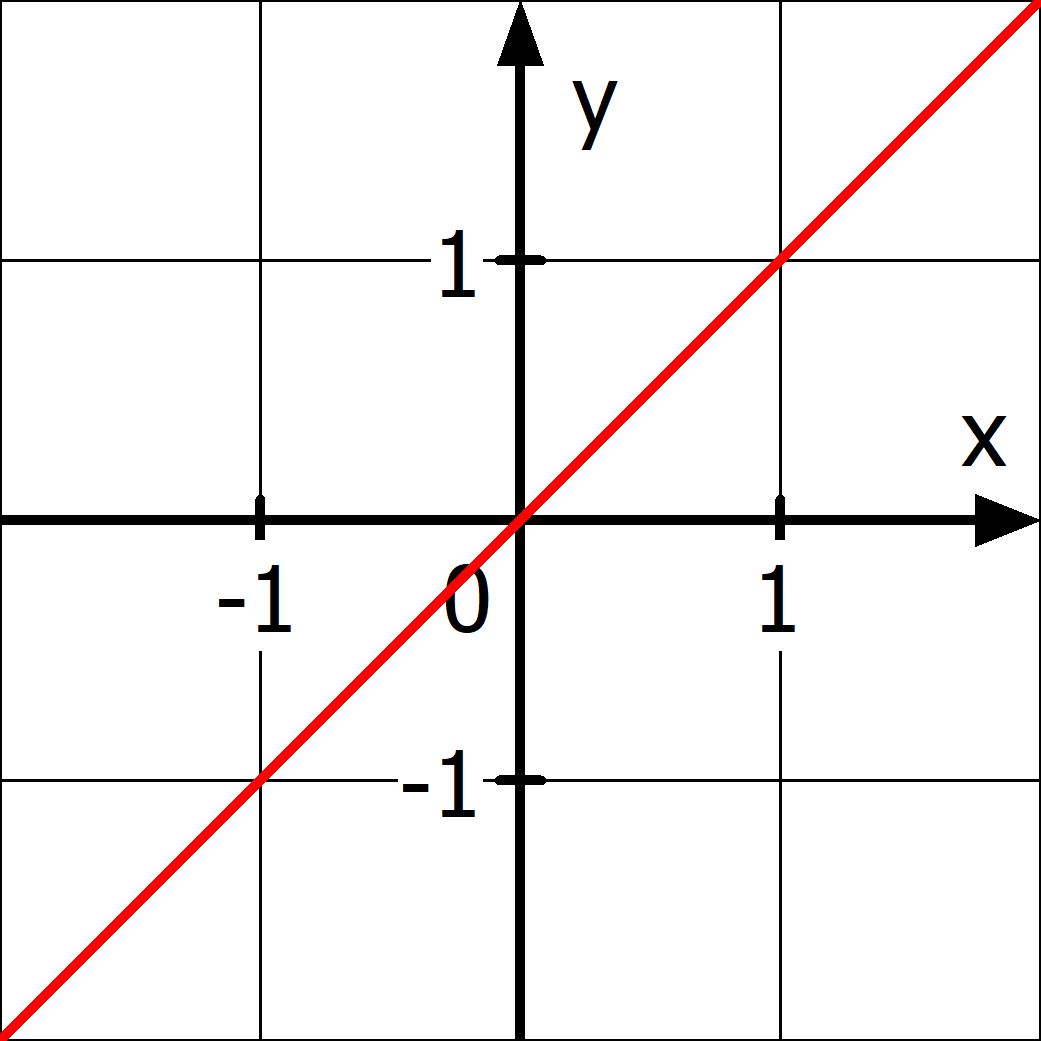
\includegraphics[width=\linewidth]{\ganzFkt/pics/potenzGerade.png}
	\end{minipage}%

	\bigskip

	\begin{minipage}{0.65\textwidth}
		\centering\Large\textcolor{loes}{Gerade Hochzahlen: \(x^2,\ x^4,\ x^6,\ \dots\)}

			\textcolor{loes}{Parabelförmig}

			\textcolor{loes}{Achsensymmetrie zur y-Achse}

			\textcolor{loes}{\(f(x)\xrightarrow{\hphantom{\ }x\to-\infty\hphantom{\ }}\infty\)}

			\textcolor{loes}{\(f(x)\xrightarrow{\hphantom{\ }x\to\infty\hphantom{\ }}\infty\)}
	\end{minipage}%
	\begin{minipage}{0.35\textwidth}
		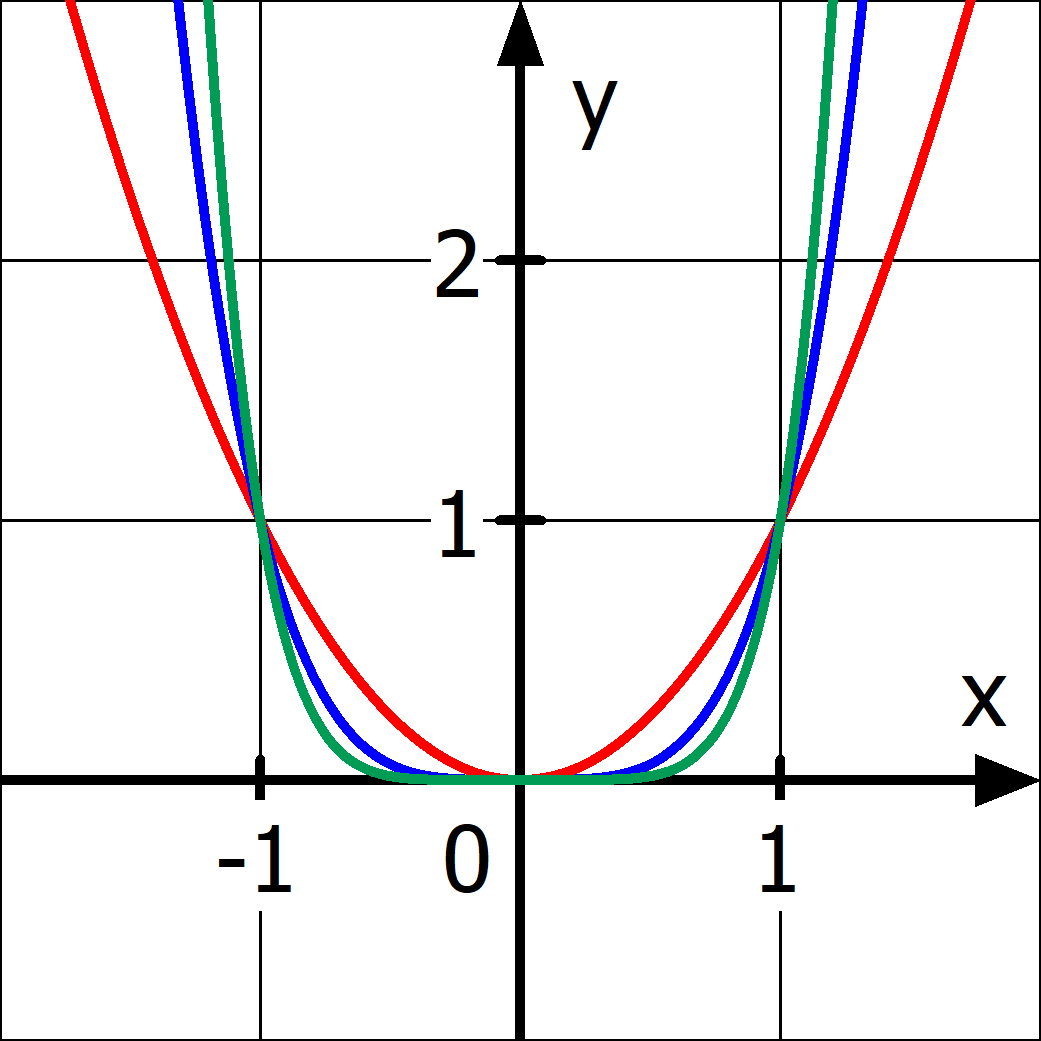
\includegraphics[width=\linewidth]{\ganzFkt/pics/potenzGeradeHZ.png}
	\end{minipage}%

	\bigskip

	\begin{minipage}{0.65\textwidth}
		\centering\Large\textcolor{loes}{Ungerade Hochzahlen (größer 1): \(x^3,\ x^5,\ x^7,\ \dots\)}

			\textcolor{loes}{S-förmig}

			\textcolor{loes}{Punktsymmetrie zum Ursprung}

			\textcolor{loes}{\(f(x)\xrightarrow{\hphantom{\ }x\to-\infty\hphantom{\ }}-\infty\)}

			\textcolor{loes}{\(f(x)\xrightarrow{\hphantom{\ }x\to\infty\hphantom{\ }}\infty\)}
	\end{minipage}%
	\begin{minipage}{0.35\textwidth}
		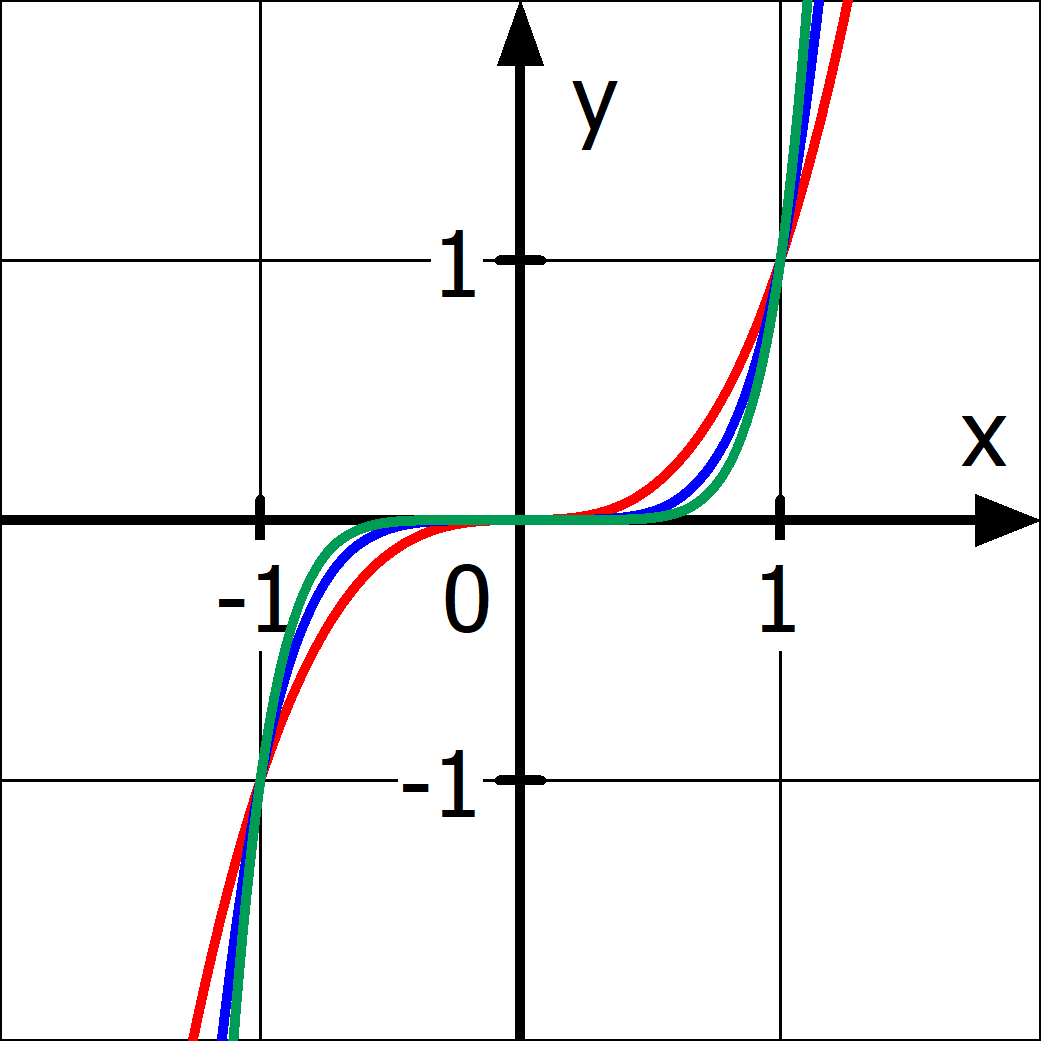
\includegraphics[width=\linewidth]{\ganzFkt/pics/potenzUngeradeHZ.png}
	\end{minipage}%
\end{minipage}
\newpage
%%%%%%%%%%%%%%%%%%%%%%%%%%%%%%%%%%%%%%%%%%%%%%%%%%%%%%%%%%%%%%%%%%%%%%%%%%%%%%%%%%%%%%%%%%%%%%%%%%%%%%%%%%%%%%%%%%%%%
\begin{Exercise}[title={Skizziere das Schaubild, gib die Symmetrie sowie das Verhalten für sehr große/kleine \(x\) an.}, label=potenzA1]

	\begin{minipage}{\textwidth}
		\begin{minipage}{0.5\textwidth}
			\begin{enumerate}[label=\alph*)]
				\item \(f(x)=-x^2\)
				\item \(g(x)=0,5x^3\)
				\item \(h(x)=2x^6\)
				\item \(i(x)=-\frac{3}{2}x^5\)
			\end{enumerate}
		\end{minipage}%
		\begin{minipage}{0.5\textwidth}
			\begin{enumerate}[label=\alph*)]
				\setcounter{enumi}{4}
				\item \(j(x)=0,1x^4\)
				\item \(k(x)=-\frac{3}{5}x^7\)
				\item \(l(x)=-\sqrt{2}x^4\)
				\item \(m(x)=3x^5\)
			\end{enumerate}
		\end{minipage}%
	\end{minipage}%
\end{Exercise}
\newpage
%%%%%%%%%%%%%%%%%%%%%%%%%%%%%%%%%%%%%%%%%
\begin{Answer}[ref=potenzA1]

	Relevant ist nur, ob die Hochzahl gerade/ungerade ist sowie das Vorzeichen des Streckfaktors:

	\bigskip

	\begin{minipage}{\textwidth}
		\begin{minipage}{0.5\textwidth}\centering
			\(a\) positiv und \(n\) gerade wie \(h(x)\) und \(j(x)\)

			Parabelförmig

			Achsensymmetrie zur y-Achse

			\(f(x)\xrightarrow{\hphantom{\ }x\to-\infty\hphantom{\ }}\infty\)

			\(f(x)\xrightarrow{\hphantom{\ }x\to\infty\hphantom{\ }}\infty\)

			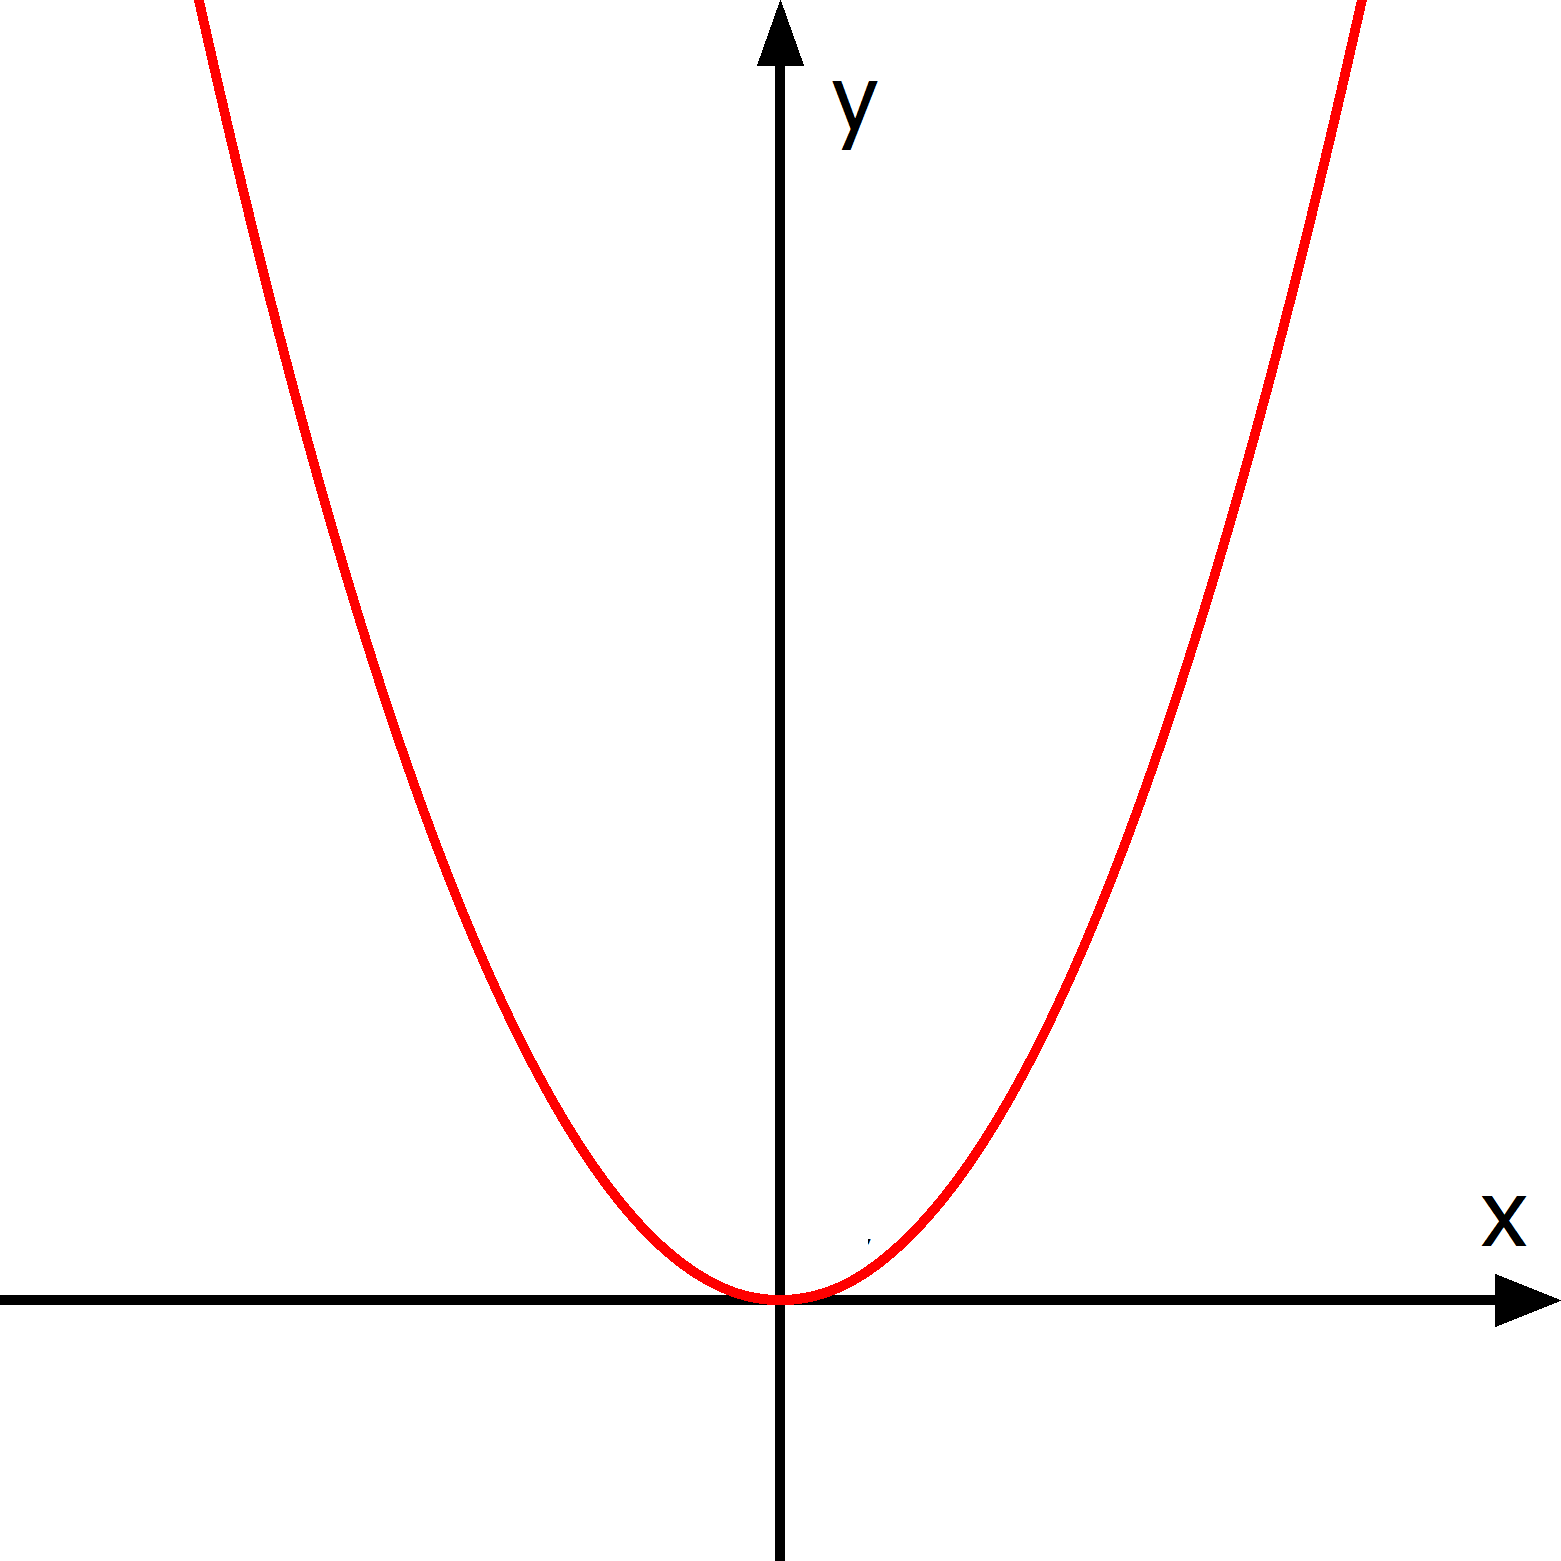
\includegraphics[width=.95\linewidth]{\ganzFkt/pics/potenzPosGerA1.png}
		\end{minipage}%
		\begin{minipage}{0.5\textwidth}\centering
			\(a\) negativ und \(n\) gerade wie \(f(x)\) und \(l(x)\)\\
			Parabelförmig

			Achsensymmetrie zur y-Achse

			\(f(x)\xrightarrow{\hphantom{\ }x\to-\infty\hphantom{\ }}-\infty\)

			\(f(x)\xrightarrow{\hphantom{\ }x\to\infty\hphantom{\ }}-\infty\)

			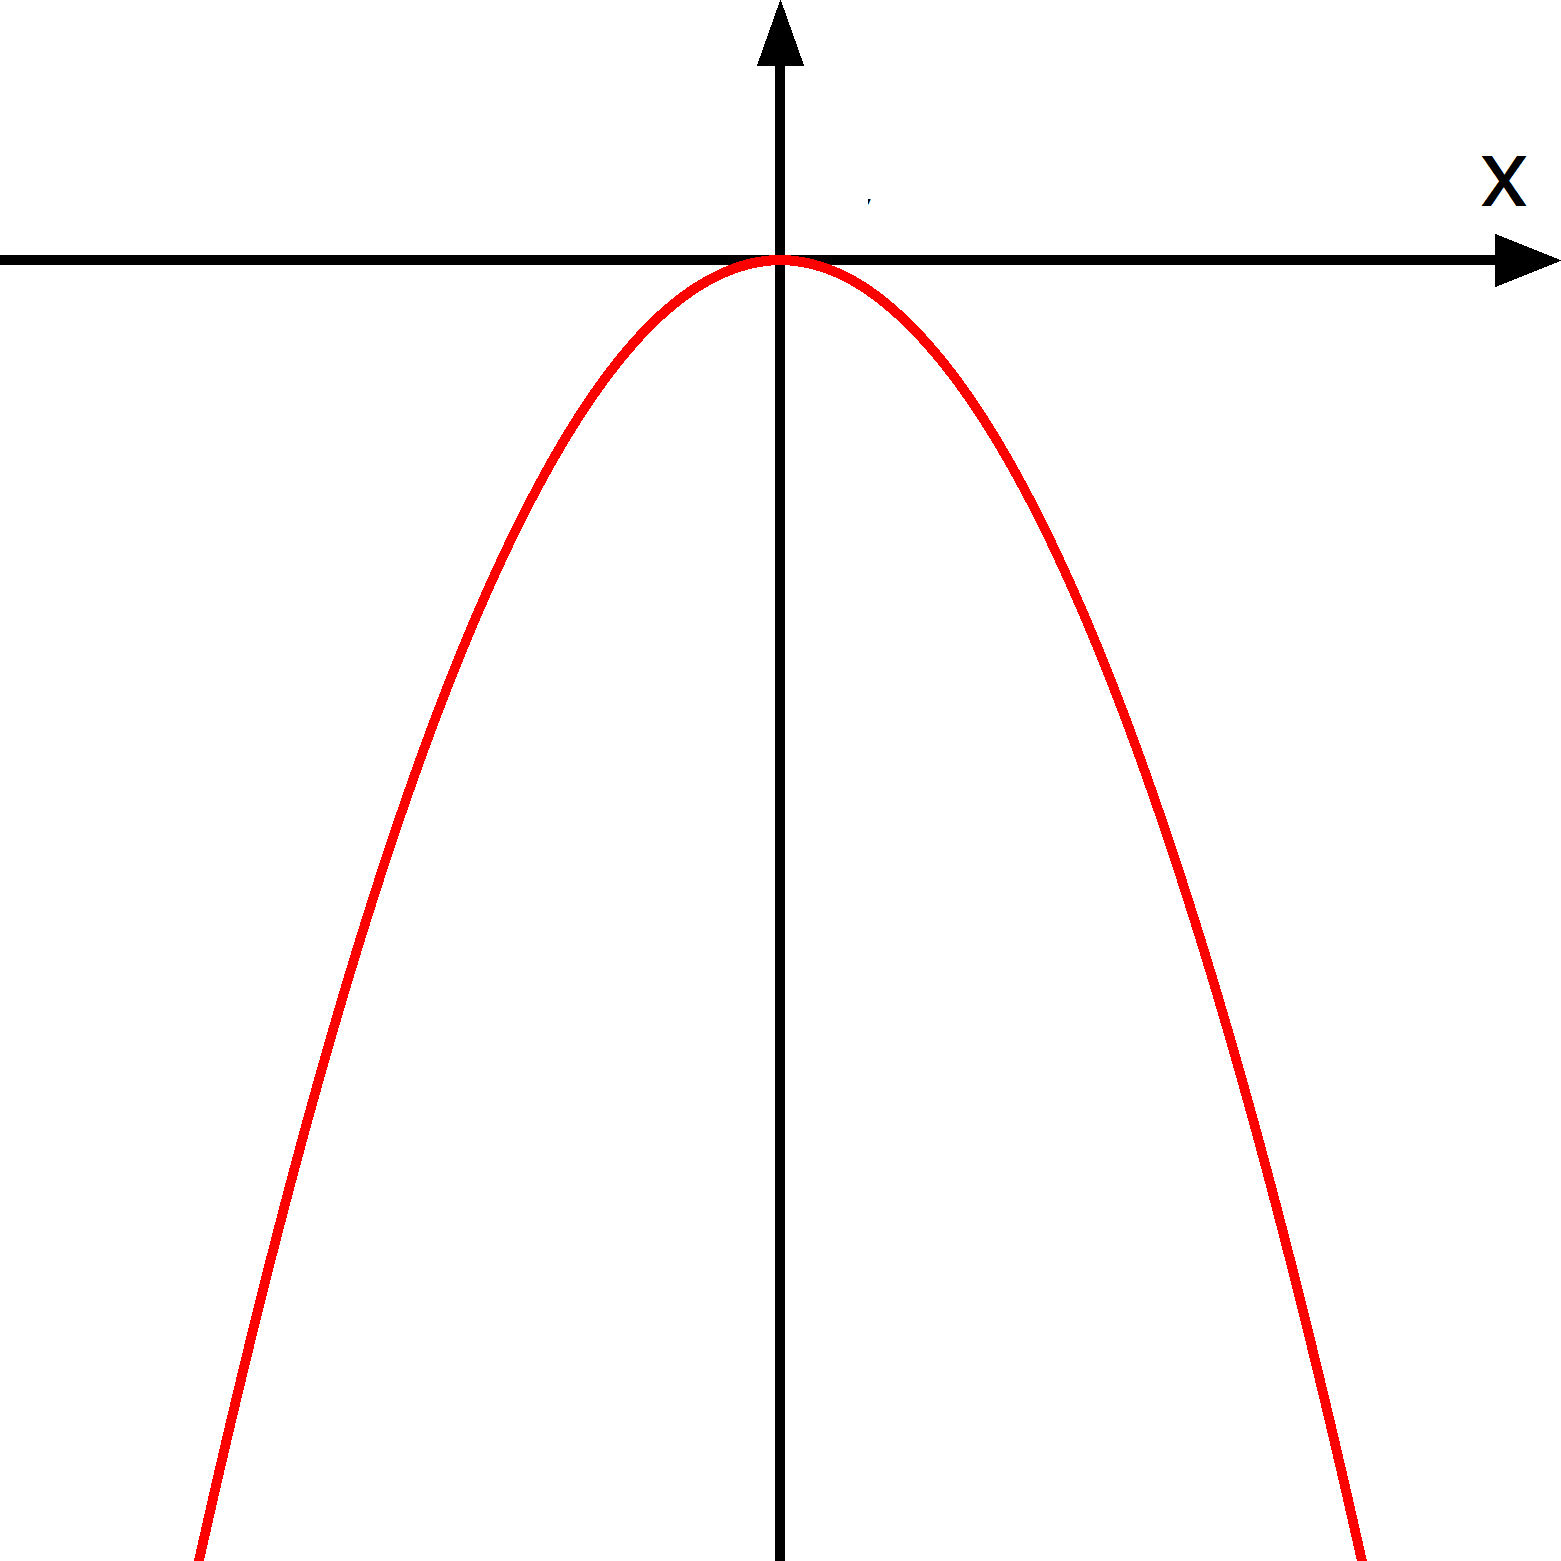
\includegraphics[width=.95\linewidth]{\ganzFkt/pics/potenzNegGerA1.png}
		\end{minipage}%

		\bigskip

		\begin{minipage}{0.5\textwidth}\centering
			\(a\) positiv und \(n\) ungerade wie \(g(x)\) und \(m(x)\)

			S-förmig

			Punktsymmetrie zum Ursprung\\
			\(f(x)\xrightarrow{\hphantom{\ }x\to-\infty\hphantom{\ }}-\infty\)

			\(f(x)\xrightarrow{\hphantom{\ }x\to\infty\hphantom{\ }}\infty\)

			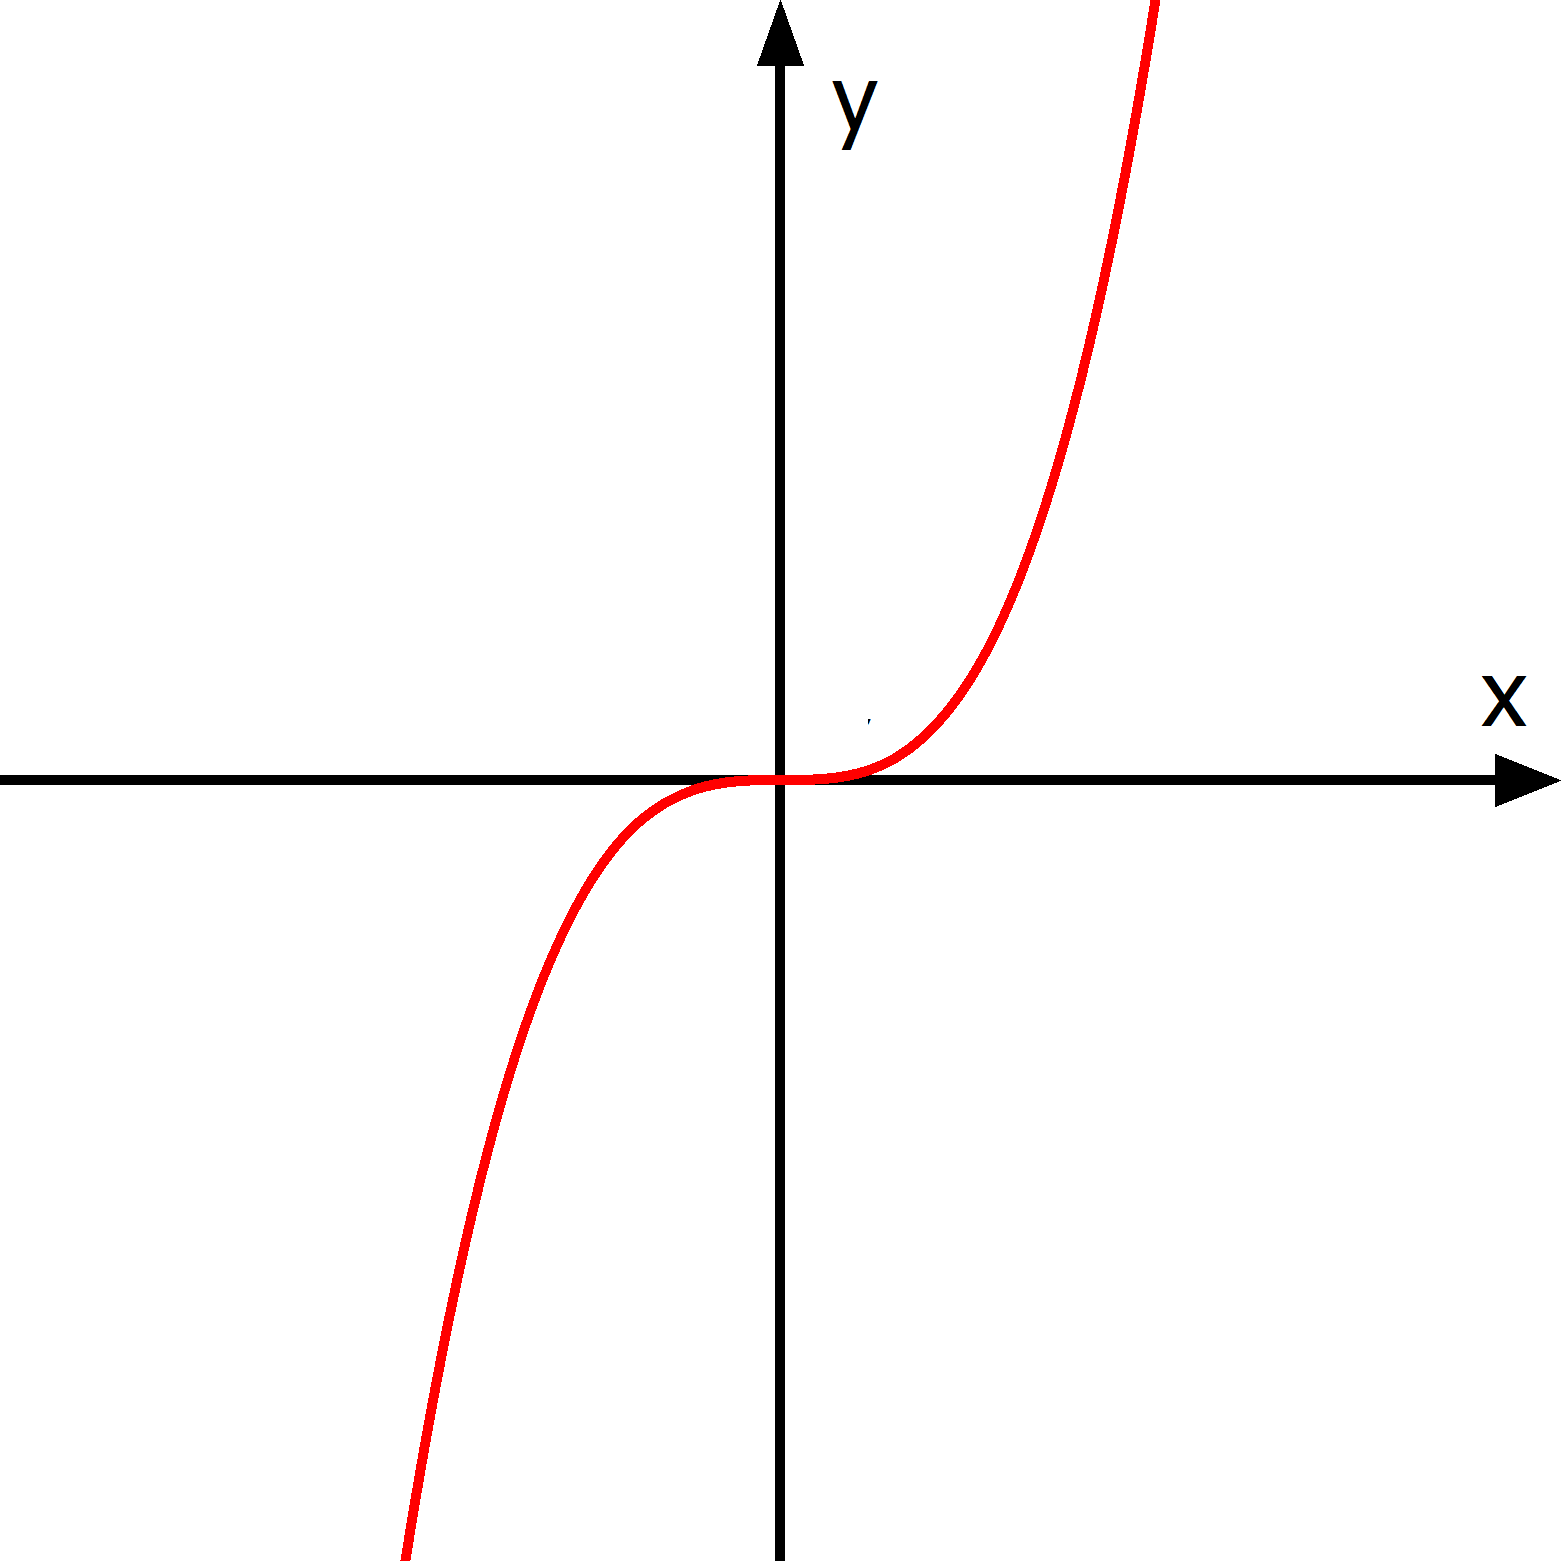
\includegraphics[width=.95\linewidth]{\ganzFkt/pics/potenzPosUngerA1.png}
		\end{minipage}%
		\begin{minipage}{0.5\textwidth}\centering
			\(a\) negativ und \(n\) ungerade wie \(i(x)\) und \(k(x)\)

			S-förmig

			Punktsymmetrie zum Ursprung

			\(f(x)\xrightarrow{\hphantom{\ }x\to-\infty\hphantom{\ }}\infty\)

			\(f(x)\xrightarrow{\hphantom{\ }x\to\infty\hphantom{\ }}-\infty\)

			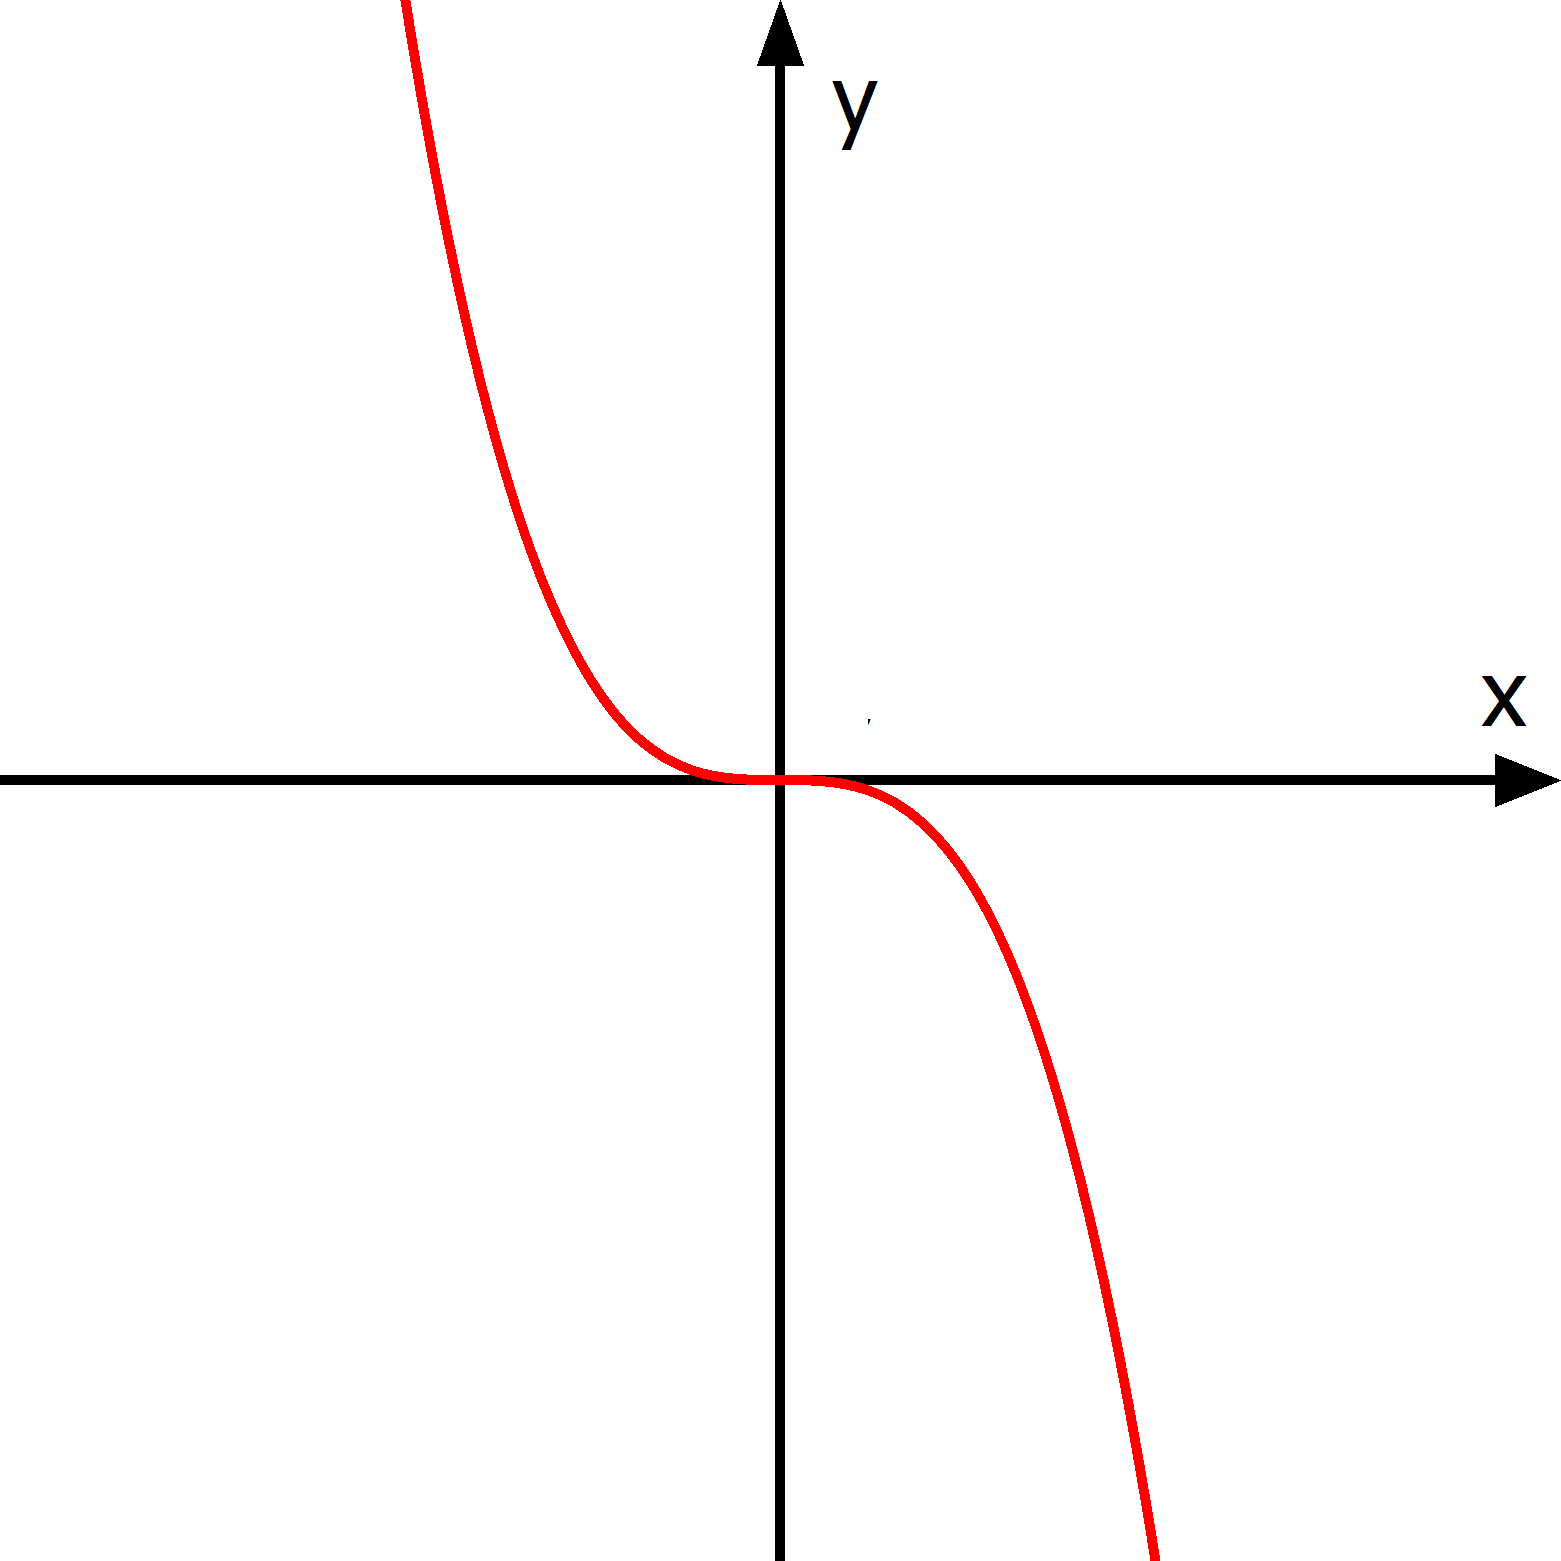
\includegraphics[width=.95\linewidth]{\ganzFkt/pics/potenzNegUngerA1.png}
		\end{minipage}%
	\end{minipage}
\end{Answer}